\باب{تغیری اصول}\شناخت{باب_تغیری_اصول} 
\حصہ{نظریہ}
 فرض کریں آپ ایک نظام،  جسے  ہیملٹنی H بیان کرتی ہو،   کی زمینی حال توانائی   \عددی{E_{gs}}   کا حساب کرنا چاہتے ہیں لیکن آپ  (غیر تابع وقت) مساوات شروڈنگر حال نہیں  کر پاتے۔\اصطلاح{ اصول تغیریت}\فرہنگ{اصول تغیریت}\حاشیہب{variational principle}\فرہنگ{variational principle} آپ کو   \عددی{E_{gs}}   کی  \ترچھا{بالائی حد بندی}  دیتا ہے،اور  بعض اوقات آپ کو صرف اسی سے غرض ہوگا،  اور عموماً،  ہوشیاری  سے کام لیتے ہوئے آپ بالکل ٹھیک قیمت کے قریب قیمت حاصل کر سکیں گے ۔ آئیں اس کا استعمال دیکھیں: کوئی ایک  معمول شدہ تفاعل  \عددی{\psi}   لیں ۔ میں درج ذیل  دعویٰ کرتا ہوں:
\begin{align}\label{مساوات_تغیری_دعوی}
E_{gs}\le \langle \psi |H|\psi\rangle \equiv \langle H \rangle
\end{align}
 یعنی کسی بھی (ممکنہ طور پر غلط)  حال  \عددی{\psi}  میں \عددی{ H} کی توقعاتی قیمت کی تخمین،   زمینی حال توانائی سے زیادہ ہوگی۔ یقیناً،  اگر   \عددی{\psi}  اتفاقاً  ہیجان حالات میں سے ایک  ہو،  تب\عددی{\langle H\rangle} کی قیمت  \عددی{E_{gs}}  سے تجاوز کرے گی؛ (جاننے والا) اصل نقطہ یہ ہے کہ کسی بھی تفاعل   \عددی{\psi}  کے لیے یہ درست ہوگا۔
 
\ابتدا{ثبوت}
چونکہ \عددی{ H} کے  (نامعلوم)   امتیازی تفاعلات مکمل سلسلہ دیتے ہیں،  لہٰذا ہم  \عددی{\psi} کو ان کا خطی جوڑ:\حاشیہد{اگر ہیملٹنی مقید حالات کے ساتھ  بکھر حالات   کا بھی حامل ہو، تب ہمیں مجموعہ کے ساتھ  تکمل بھی درکار ہو گا،تاہم باقی دلیل یہی رہی گی۔}
\begin{align*}
H\psi_{n}=E_{n}\psi_{n}\quad \text{\RL{جہاں}}\quad\psi=\sum_n c_{n}\psi_{n} 
\end{align*}
ہے   لکھ سکتے ہیں۔چونکہ  \عددی{\psi} معمول شدہ ہے، لہٰذا درج ذیل ہو گا
\begin{align*}
1=\langle \psi |\psi\rangle=\big\langle \sum_{m} c_{m}\psi_{m}|\sum_{n}c_{n}\psi_{n}\big\rangle=\sum_{m}\sum_{n}c_{m}^{*}c_{n}\langle \psi_{m}|\psi_{n}\rangle=\sum_{n}\abs{c_{n}}^{2} 
\end{align*}

 (جہاں فرض کیا گیا ہے کہ  امتیازی تفاعلات    معیاری عمود  شدہ ہیں: \عددی{\langle \psi_{m}|\psi_{n}\rangle=\delta_{mn}})۔    ساتھ ہی درج ذیل ہوگا۔
\begin{align*}
\langle H \rangle=\big\langle \sum_{m} c_{m}\psi_{m}|H\sum_{n}c_{n}\psi_{n}\big\rangle=\sum_{m}\sum_{n}c_{m}^{*}E_{n}c_{n}\langle \psi_{m}|\psi_{n}\rangle=\sum_{n}E_{n}\abs{c_{n}}^{2}
 \end{align*}

  لیکن    تعریف  کی رو سے،  زمینی حال توانائی کم سے کم امتیازی قیمت ہوگی،  لہٰذا \عددی{E_{gs}\le E_{n}} ہوگا، جس کے تحت درج ذیل ہوگا۔
\begin{align*}
\langle H \rangle \ge E_{gs}\sum_{n}\abs{c_{n}}^{2}=E_{gs} 
\end{align*}
ہم یہی ثابت کرنا چاہتے تھے۔
 \انتہا{ثبوت}
\ابتدا{مثال}
فرض  کریں   ہم یک بُعدی ہارمونی مرتعش:
\begin{align*}
H=-\frac{\hslash^{2}}{2m}\frac{\dif^{\,2}}{\dif{x^{2}}}+\frac{1}{2}m\omega^{2}x^{2} 
\end{align*}


 کی زمینی حال توانائی جاننا چاہتے ہیں ۔ یقیناً، ہم اس کا ٹھیک ٹھیک جواب جانتے ہیں ( مساوات  \حوالہ{مساوات_شروڈنگر_ہارمونی_حالات}):  \عددی{E_{gs}=(1/2)\hslash\omega}؛  جس سے  اس ترکیب کو  پرکھا  جا سکتا ہے۔ ہم گاوسی تفاعل:
 \begin{align}\label{مساوات_تغیری_گاوسی_آزمائشی_تفاعل}
\psi(x)=Ae^{-bx^{2}} 
\end{align}


 
کو اپنا  "آزمائشی"  تفاعل موج منتخب کرتے ہیں،  جہاں \عددی{b }ایک مستقل ہے،  اور\عددی{ A} کو معمول زنی
\begin{align}
1=\abs{A}^{2}\int_{-\infty}^{+\infty}e^{-2bx^{2}}\dif{x}=\abs{A}^{2}\sqrt{\frac{\pi}{2b}}\Rightarrow A=\big (\frac{2b}{\pi}\big )^{1/4} 
\end{align}
 تعین کرتی ہے۔ اب 
 \begin{align}
 \langle H \rangle=\langle T \rangle + \langle V \rangle
\end{align}
 
ہے،  جبکہ یہاں
\begin{align}
\langle T \rangle=-\frac{\hslash^{2}}{2m}\abs{A}^{2}\int_{-\infty}^{+\infty}e^{-bx^{2}}\frac{\dif^{\,2}}{\dif{x^{2}}}(e^{-bx^{2}})\dif{x}=\frac{\hslash^{2}b}{2m} 
\end{align}

 اور
\begin{align*}
\langle V\rangle=\frac{1}{2}m\omega^{2}\abs{A}^{2}\int_{-\infty}^{+\infty}e^{-2bx^{2}}x^{2}\dif{x}=\frac{m\omega^{2}}{8b} 
\end{align*}

لہٰذا  درج ذیل ہوگا۔
\begin{align}
 \langle H \rangle=\frac{\hslash^{2}b}{2m}+\frac{m\omega^{2}}{8b} 
\end{align}

مساوات  \حوالہ{مساوات_تغیری_دعوی} کے تحت  کسی بھی \عددی{ b} کے لئے یہ  \عددی{E_{gs}}  سے تجاوز کرے گا؛ سخت سے سخت حد بندی کی خاطر ہم  \عددی{ \langle H\rangle}  کی کم سے کم قیمت تلاش  کرتے ہے:
\begin{align*}
\frac{\dif}{\dif b}\langle H\rangle=\frac{\hslash^{2}}{2m}-\frac{m\omega^{2}}{8b^{2}}=0\Rightarrow b=\frac{m\omega}{2\hslash} 
\end{align*}

 اس کو واپس  \عددی{ \langle H\rangle } میں پر کرتے ہوئے درج ذیل حاصل ہوگا۔
 \begin{align}
\langle H\rangle _{\text{\RL{کمتر}}} =\frac{1}{2}\hslash\omega
\end{align}
 یہاں ہم بالکل ٹھیک زمینی حال توانائی حاصل کر پائے ہیں،   جو حیرانی کی بات نہیں ،  چونکہ میں نے (اتفاقاً)  ایسا آزمائشی تفاعل منتخب کیا جس کا روپ ٹھیک اصل  زمینی حال( مساوات \حوالہ{مساوات_شروڈنگر_معمول_شدہ_حال_صفر}) کی طرح ہے۔  تاہم،  گاوسی کے ساتھ کام کرنا انتہائی آسان ثابت ہوتا ہے،  لہٰذا یہ ایک مقبول  آزمائشی  تفاعل ہے،  اور وہاں بھی استعمال کیا جاتا ہے جہاں  اصل  زمینی حال کے ساتھ اس کی کوئی مشابہت نہ ہو۔
 \انتہا{مثال}
\ابتدا{مثال}
فرض کرے ہم ڈیلٹا  تفاعل مخفیہ:
\begin{align*}
 H=-\frac{\hslash^{2}}{2m}\frac{\dif^{\,2}}{\dif{x^{2}}}-\alpha\delta(x)
\end{align*}

 کی زمینی حال توانائی جاننا چاہتے ہیں۔  ہمیں ٹھیک جواب (مساوات \حوالہ{مساوات_شروڈنگر_مقید_حال_ڈیلٹا}):   \عددی{E_{gs}=-m\alpha^{2}/2\hslash^{2}} یہاں بھی معلوم ہے۔ پہلے کی طرح،  ہم گاوسی آزمائشی تفاعل (مساوات \حوالہ{مساوات_تغیری_گاوسی_آزمائشی_تفاعل})   کا انتخاب کرتے ہیں۔ ہم معمول زنی کر چکے ہیں،  اور  \عددی{\langle T\rangle}  کا حساب کر چکے ہیں؛   ہمیں صرف درجہ ذیل درکار ہے۔
\begin{align*}
\langle V\rangle=-\alpha\abs{A}^{2}\int_{-\infty}^{+\infty}e^{-2bx^{2}}\delta(x)\dif{x}=-\alpha\sqrt{\frac{2b}{\pi}} 
\end{align*}

 ظاہر ہے
 \begin{align}
\langle H\rangle=\frac{\hslash^{2}b}{2m}-\alpha\sqrt{\frac{2b}{\pi}} 
\end{align}

 اور ہم جانتے ہیں کہ یہ تمام  \عددی{b} کے لیے  \عددی{ E_{gs}}  سے تجاوز کرے گا۔ اس کی کم سے کم قیمت تلاش کرتے ہے
\begin{align*}
\frac{\dif}{\dif b}\langle H\rangle=\frac{\hslash^{2}}{2m}-\frac{\alpha}{\sqrt{2\pi b}}=0\Rightarrow b=\frac{2m^{2}\alpha^{2}}{\pi\hslash^{4}} 
\end{align*}

 لہٰذا 
 \begin{align}
\langle H\rangle _{\text{\RL{کمتر}}} =-\frac{m\alpha^{2}}{\pi\hslash^{2}} 
\end{align}

 ہو گا، جو  یقیناً \عددی{ E_{gs}}  سے  معمولی   زیادہ ہے(چونکہ \عددی{\pi>2} ہے)۔
 \انتہا{مثال}
 
میں نے کہا آپ کسی بھی  (معمول شدہ)  آزمائشی تفاعل  \عددی{\psi}  کا انتخاب کر سکتے ہیں،  جو ایک لحاظ سے درست ہے۔ البتہ،  \ترچھا{ غیر استمراری}  تفاعلات کے دہرا تفرق ( جو \عددی{ \langle T \rangle} کی قیمت حاصل کرنے کے لیے درکار ہوگا) کو معنی خیز مطلب مختص کرنے کے لیے انوکھے چال چلنا ہوگا۔ ہاں،   اگر آپ محتاط رہیں  تو،  استمراری تفاعلات جن میں بل پائے جاتے ہوں  کا استعمال  نسبتاً آسان ہے۔ اگلی مثال میں ان سے نمٹنا   دکھایا گیا ہے۔\حاشیہد{ایسا تفاعل  (مثلاً گاوسی)  جو کنویں سے باہر سرکتا ہو استعمال کرنا بے مقصد ہے، چونکہ آپ  \عددی{\langle V\rangle=\infty} حاصل کرتے ہیں  اور مساوات \حوالہ{مساوات_تغیری_دعوی}  کچھ نہیں بتاتی۔}


\ابتدا{مثال}
آزمائشی "تکونی"  تفاعل موج (شکل \حوالہ{شکل_تغیریت_لامتناہی_کنواں_تکونی_موج}):
\begin{align}\label{مساوات_تغیریت_آزمائشی_تکونی_تفاعل}
\psi(x)=\begin{cases} Ax & 0\le x\le a/2\\
A(a-x) & a/2\le x\le a\\
0 & \text{\RL{دیگر صورت}} \end{cases} 
\end{align}

 استعمال کرتے ہوئے یک بُعدی لا متناہی چوکور کنویں کی زمینی حال توانائی کی بالائی حد بندی تلاش کریں،  جہاں \عددی{ A}  معمول زنی سے تعین کیا جائے گا۔
\begin{align}
1=\abs{A}^{2}\big [\int_{0}^{a/2} x^{2}\dif{x}+\int_{a/2}^{a}(a-x)^{2}\dif{x} \big ]=\abs{A}^{2}\frac{a^{3}}{12}\Rightarrow A=\frac{2}{a}\sqrt{\frac{3}{a}} 
\end{align}
%
\begin{figure}
 \centering
 \begin{minipage}{0.45\textwidth}
 \centering
\begin{tikzpicture}[x={0.75cm},y={0.75cm}]
 \fill[path fading=west,color=lgray] (-0.25,0) rectangle (0,3.75);
\fill[path fading=east,color=lgray] (5,0) rectangle (5.25,3.75);
\draw[-stealth] (-0.5,0) -- (5.75,0)node[below]{$x$};
\draw[-stealth] (0,-0.25) -- (0,4)node[left]{$\psi(x)$};
\draw[very thick](0,0) -- (2.5,3) -- (5,0) node[below]{$a$};
\draw[](2.5,0.1) -- (2.5,-0.1) node[below]{$a/2$};
\draw[](5,0) -- (5,3.75);
\end{tikzpicture}
 \caption{لامتناہی چوکور کنواں کے لئے آزمائشی تکونی تفاعل موج (مساوات \حوالہ{مساوات_تغیریت_آزمائشی_تکونی_تفاعل})۔} 
 \label{شکل_تغیریت_لامتناہی_کنواں_تکونی_موج}
 \end{minipage}\hfill
 \begin{minipage}{0.45\textwidth}
  \centering
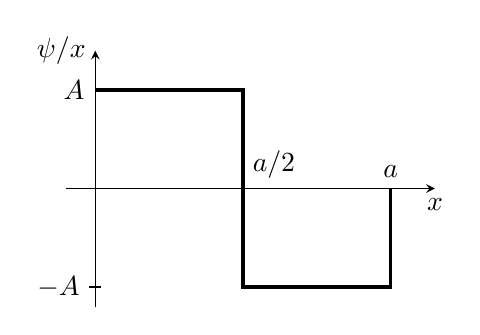
\begin{tikzpicture}[x={0.75cm}] 
\draw[-stealth] (-0.5,0) -- (5.75,0)node[below]{$x$};
\draw[-stealth] (0,-1.5) -- (0,1.75)node[left]{$\dif\psi/\dif x$};
\draw[very thick](0,1.25) node[left]{$A$} -- (2.5,1.25) -- (2.5,-1.25) -- (5,-1.25) -- (5,0) node[above]{$a$};
\draw[] (-0.1,-1.25) node[left]{$-A$} -- (0.1,-1.25);
\draw[] (2.5,0) node[above right]{$a/2$};
\end{tikzpicture} 
\caption{تکونی تفاعل موج (شکل \حوالہ{شکل_تغیریت_لامتناہی_کنواں_تکونی_موج}) کا تفرق۔} 
\label{شکل_تغیریت_لامتناہی_کنواں_تکونی_موج_تفرق} 
\end{minipage}
\end{figure} 
 
جیسا شکل \حوالہ{شکل_تغیریت_لامتناہی_کنواں_تکونی_موج_تفرق} میں دکھایا گیا ہے یہاں درجہ ذیل ہوگا۔
\begin{align*}
\frac{\dif{\psi}}{\dif{x}}=\begin{cases} A & 0<x<a/2\\
-A & a/2<x<a\\
0& \text{\RL{دیگر صورت}} \end{cases} 
\end{align*}

 

  سیڑھی تفاعل کا تفرق ایک  ڈیلٹا  تفاعل ہے ( سوال   \حوالہ{سوال_شروڈنگر_تفاعلات_برابر}-ب دیکھیں):
\begin{align}
\frac{\dif^{\,2}{\psi}}{\dif{x^{2}}}=A\delta(x)-2A\delta(x-a/2)+A\delta(x-a)
\end{align}

 لہٰذا درج ذیل ہوگا ۔
\begin{align} 
\langle H \rangle &= -\frac{\hslash^{2}A}{2m}\int[\delta(x)-2\delta(x-a/2)+\delta(x-a)]\psi(x)\dif{x}\nonumber\\
&= -\frac{\hslash^{2}A}{2m}[\psi(0)-2\psi(a/2)+\psi(a)]=\frac{\hslash^{2}A^{2}a}{2m}=\frac{12\hslash^{2}}{2ma^{2}}
\end{align}
 ٹھیک زمینی حال توانائی \عددی{E_{gs}=\frac{\pi^{2}\hslash^{2}}{2ma^{2}}} (مساوات  \حوالہ{مساوات_شروڈنگر_لامتناہی_چکور_کنواں_توانائیاں}) ہے، لہٰذا یہ مسئلہ کار آمد ہے ( \عددی{12>\pi^{2}})۔
 \انتہا{مثال}
%===================
اصول تغیریت انتہائی طاقتور اور استعمال کے نقطہ نظر سے شرمناک حد تک آسان ہے۔ کسی پیچیدہ سالمہ کی زمینی حال توانائی جاننے کے لئے ماہر کیمیا    متعدد مقدار معلوم  والا   آزمائشی تفاعل موج منتخب کر کے  ان مقدار معلوم  کی قیمتیں تبدیل کرتے ہوئے \عددی{ \langle H \rangle} کی سب سے کم ممکنہ قیمت تلاش کرتا ہے۔ اصل تفاعل موج کے ساتھ \عددی{\psi} کی کوئی مشابہت نہ  ہونے کی صورت میں بھی آپ کو \عددی{ E_{gs}}  کی حیرت کن حد تک درست قیمت حاصل ہوگی۔ ظاہر ہے،  اگر آپ \عددی{\psi}  کو اصل  تفاعل کے جتنا  زیادہ قریب منتخب کر پائیں،  اتنا بہتر ہوگا۔ اس ترکیب کے ساتھ صرف ایک  مسئلہ  ہے:  آپ کبھی بھی نہیں  جان  سکتے کہ آپ ہدف  کے کتنے قریب ہیں؛  آپ صرف  بالائی حد بندی جان پاتے ہو۔\حاشیہد{عملاً یہ بہت بڑا مسئلہ نہیں  اور بعض اوقات درستگی کا اندازہ لگایا جا سکتا  ہے۔ زمینی حال ہیلیم کو کئی با معنی ہندسوں تک اس طرح حل کیا گیا ہے۔  }  مزید،  اس روپ میں یہ ترکیب صرف زمینی حال کے لیے کارآمد ہے (البتہ سوال  \حوالہ{سوال_تغیریت_ترکیب_کارآمد_پہلا_ہیجان}  دیکھیں)۔
%===========

\ابتدا{سوال}
درجہ ذیل مخفیہ کی  زمینی حال توانائی جاننے کے لئے   گاوسی آزمائشی تفاعل (مساوات \حوالہ{مساوات_تغیری_گاوسی_آزمائشی_تفاعل})  کی سب  سے کم بالائی حد بندی تلاش کریں۔
\begin{enumerate}[a.]
\item
 خطی مخفیہ \عددی{V(x)=\alpha\abs{x}}؛
\item
 چو طاقت  مخفیہ \عددی{V(x)=\alpha x^{4}}
\end{enumerate}
\انتہا{سوال}
 \ابتدا{سوال}
 یک بُعدی ہارمونی مرتعش  کے    \عددی{E_{gs}}  کی بہترین حد بندی  درج ذیل روپ کا  آزمائشی تفاعل موج
\begin{align*}
\psi(x)=\frac{A}{x^{2}+b^{2}} 
\end{align*}
 استعمال کرکے تلاش کریں، جہاں \عددی{A}  معمول زنی سے تعین ہوگا  اور  \عددی{b} قابل تبدیل مقدار معلوم ہے۔
 \انتہا{سوال}
 \ابتدا{سوال}
 ڈیلٹا تفاعل مخفیہ  \عددی{V(x)=-\alpha\delta(x)}   کی  \عددی{E_{gs}} کی بہترین بالائی حد بندی کو تکونی آزمائشی تفاعل (مساوات  \حوالہ{مساوات_تغیریت_آزمائشی_تکونی_تفاعل}،  لیکن جس کا وسط مبدا پر ہو)  استعمال کرکے تلاش کریں۔  یہاں \عددی{ a}  قابل تبدیل مقدار معلوم ہے۔
 \انتہا{سوال}
\ابتدا{سوال}\شناخت{سوال_تغیریت_ترکیب_کارآمد_پہلا_ہیجان}
\begin{enumerate}[a.]
\item
 اصول تغیریت کا  درج ذیل ضمنی  نتیجہ  ثابت کریں: اگر \عددی{\langle \psi | \psi_{gs} \rangle =0} ہو، تب \عددی{\langle H \rangle \ge E_{fe}} ہوگا،  جہاں پہلے  ہیجان حال کی توانائی  \عددی{E_{fe}}  ہے۔ 
 
 یوں، اگر ہم کسی طرح   ایسا    آزمائشی تفاعل تلاش  کر  سکیں جو  اصل زمینی حال کو عمودی ہو، تب ہم  \ترچھا{پہلے ہیجان حال} کی بالائی حد بندی جان سکیں گے۔  چونکہ ہم  زمینی حال تفاعل  \عددی{\psi_{gs}}   (غالباً) نہیں جانتے،  لہٰذا عموماً  یہ کہنا مشکل ہوگا کہ    \عددی{\psi}  ہمارے آزمائشی تفاعل \عددی{\psi_{gs}} کو عمودی ہوگا۔ ہاں،  اگر \عددی{ x} کے لحاظ سے مخفیہ   \عددی{V(x)}      \ترچھا{جفت} تفاعل ہو،  تب زمینی حال بھی جفت ہوگا، اور یوں  کوئی بھی \ترچھا{ طاق} آزمائشی تفاعل خود بخود اس    ضمنی  نتیجہ کے شرط پر پورا اترے گا۔
 \item
   آزمائشی تفاعل:
\begin{align*}
\psi(x)=Axe^{-bx^{2}} 
\end{align*}
 استعمال کرتے ہوئے یک بُعدی ہارمونی مرتعش کے پہلے  ہیجان حال کی  بہترین بالائی حد بندی تلاش کریں۔
 \end{enumerate}
 \انتہا{سوال}
 \ابتدا{سوال}
\begin{enumerate}[a.]
\item
 اصول تغیریت استعمال کرکے ثابت کریں کہ رتبہ اول غیر انحطاطی نظریہ اضطراب ہر صورت زمینی حال توانائی کی قیمت سے تجاوز کرے گا   (یا کم از  کم کبھی بھی اس سے کم قیمت نہیں دے گا)۔
 \item
  آپ جزو-الف جانتے ہوئے توقع کریں گے کہ زمینی حال کی دو رتبی تصحیح لازماً منفی ہوگی۔ مساوات  \حوالہ{مساوات_غیر_اضطراب_دوم_رتبی_نتیجہ} کا معائنہ کرتے ہوئے تصدیق کریں کہ ایسا ہی ہوگا۔
  \end{enumerate}
\انتہا{سوال}


\حصہ{ہیلیم کا زمینی حال} 
ہیلیم جوہر  (شکل \حوالہ{شکل_تغیریت_ہیلیم_جوہر}) کے مرکزہ میں دو پروٹان ( اور دو نیوٹران  جو ہمارے مقصد سے غیر متعلقہ ہیں)   پائے جاتے ہیں اور مرکزہ کے گرد مدار میں دو الیکٹران حرکت کرتے ہیں۔
(مہین ساخت اور باریک تصحیح  نظر انداز کرتے ہوئے)  اس نظام کی ہیملٹنی درج ذیل ہوگی۔
\begin{align}\label{مساوات_تغیریتی_ہیلیم_ہیملٹنی}
H=-\frac{\hslash^{2}}{2m}(\nabla_{1}^{2}+\nabla_{2}^{2})-\frac{e^{2}}{4\pi\epsilon_{0}}\big (\frac{2}{r_{1}}+\frac{2}{r_{2}}-\frac{1}{\abs{\kvec{r}_{1}-\kvec{r}_{2}}}\big )
\end{align}
 
\begin{figure}
 \centering
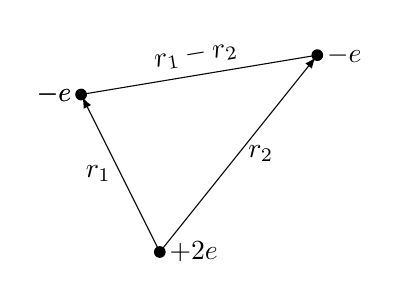
\begin{tikzpicture} \draw[-latex,shorten >=1pt] (0,0) node[right]{$+2e$} node[circle, fill=black,inner sep=1.5pt]{} -- (-1,2) node[left]{$-e$} node[pos=0.5,left]{$\kvec{r}_1$};
\draw[] (-1,2) node[left]{$-e$} node[circle, fill=black,inner sep=1.5pt]{} -- (2,2.5) node[right]{$-e$} node[pos=0.5,above,sloped]{$\abs{\kvec{r}_1-\kvec{r}_2}$} node[circle, fill=black,inner sep=1.5pt]{};
\draw[-latex,shorten >=1pt] (0,0) -- (2,2.5) node[pos=0.5,right]{$\kvec{r}_2$};
\end{tikzpicture} 
\caption{ہیلیم جوہر۔} 
\label{شکل_تغیریت_ہیلیم_جوہر} 
\end{figure} 

ہم نے زمینی حال توانائی   \عددی{E_{gs}}  کا حساب کرنا ہے ۔ طبیعی طور پر یہ دونوں الیکٹران اکھاڑنے کے لیے درکار توانائی کو ظاہر کرتی ہے۔ (   \عددی{E_{gs}}   جانتے ہوئے،  ہم  \ترچھا{ایک}  الیکٹران اکھاڑنے کے لیے درکار  "بارداریتی  توانائی"   معلوم کر سکتے ہیں (سوال \حوالہ{سوال_تغیریت_بارداریتی_توانائی}  دیکھیں)۔   تجربہ گاہ میں ہیلیم کی زمینی حل توانائی کی قیمت کی پیمائش  انتہائی زیادہ درستگی تک کی گئی ہے۔
\begin{align}
E_{gs}&=\SI{-78.975}{\electronvolt} &&(\text{\RL{تجرباتی}})
\end{align}
 ہم نظریہ سے اس عدد کو حاصل کرنا چاہیں گے۔
 
  یہ تجسس کی بات ہے کہ ابھی تک اتنے سادہ اور اہم مسئلے کا ٹھیک حل نہیں ڈھونڈا جا سکا ہے۔\حاشیہد{ہیلیم کے کیفی  خدوخال  والے، ایسے تین جسمی مسئلے پائے جاتے ہیں جن کا ٹھیک ٹھیک حل حاصل کیا جا سکتا ہے، تاہم ان میں مخفیے  غیر کولمب   ہیں (سوال \حوالہ{سوال_تغیریتی_ہیلیم_نما_غیر_کولمب} دیکھیں)۔ }   الیکٹران الیکٹران دفع :
\begin{align}
V_{ee}=\frac{e^{2}}{4\pi\epsilon_{0}}\frac{1}{\abs{\kvec{r}_{1}-\kvec{r}_{2}}} 
\end{align}
 مسئلہ پیدا کرتا ہے۔ اس جزو کو نظر انداز کرنے سے  \عددی{H} دو  ہائیڈروجن ہیملٹنیوں  میں علیحدہ    علیحدہ ہوتا ہے  (تاہم   مرکزوی  بار \عددی{ e} کی بجائے  \عددی{2e}  ہوگا)؛  ٹھیک ٹھیک حل ہائیڈروجنی تفاعلات موج کا حاصل ضرب:
\begin{align}\label{مساوات_تغیریتی_ہیلیم_علیحدہ}
\psi_{0}(\kvec{r}_{1},\kvec{r}_{2})\equiv \psi_{100}(\kvec{r}_{1})\psi_{100}(\kvec{r}_{2})=
\frac{8}{\pi a^{3}}e^{-2(r_{1}+r_{2})/a}
\end{align}
 ہو گا، اور توانائی  \عددی{8E_1=\SI{-109}{\electronvolt}}  الیکٹران وولٹ  (مساوات \حوالہ{مساوات_متماثل_ہیلیم_توانائی_الف})ہوگی ۔\حاشیہد{یہاں \عددی{a} سادہ رداس بوہر ہے اور   \عددی{n} ویں بوہر توانائی \عددی{E_n=-13.6/n^2\,\si{\electronvolt}} ہے؛ یاد رہے کہ ایک مرکزہ جس کا جوہری عدد \عددی{Z} ہو، کے لئے \عددی{E_n\to Z^2E_n} اور \عددی{a\to a/Z} ہوں گے (سوال \حوالہ{سوال_تین_ابعادی_ہائیڈروجنی_جوہر})۔مساوات \حوالہ{مساوات_تغیریتی_ہیلیم_علیحدہ}  کے ساتھ وابستہ چکری تشکیل غیر تشاکلی (یک تا) ہو گی۔}  یہ   \عددی{\SI{-79}{\electronvolt}}   سے بہت  مختلف  ہے،   تاہم یہ ابھی  ابتدا  ہے ۔
 
  ہم  \عددی{\psi_0} کو  آزمائشی تفاعل  موج لے کر    \عددی{E_{gs}}  کی بہتر تخمین  اصول تغیریت سے حاصل کرتے ہیں۔ چونکہ یہ  ہیملٹنی کے زیادہ تر حصے  کا امتیازی تفاعل ہے:
\begin{align}
H\psi_{0}=(8E_{1}+V_{ee})\psi_{0} 
\end{align}
 لہٰذا یہ  بہت  بہتر انتخاب ہے۔یوں درج ذیل ہو گا 
\begin{align}
\langle H \rangle=8E_{1}+\langle V_{ee}\rangle
\end{align}
 جہاں درج ذیل ہے ۔\حاشیہد{آپ  \عددی{H'=V_{ee}} لیتے ہوئے مساوات \حوالہ{مساوات_تغیریت_تکمل_آئے} کا مفہوم اول رتبی نظریہ اضطراب لے  سکتے  ہیں۔میں اس کو اس ترکیب کا غلط استعمال سمجھتا  ہوں، چونکہ  یہاں اضطراب اور غیر مضطرب ہیملٹنی ہم  پلہ  ہیں۔ اس وجہ سے میں اس کو تغیریتی حساب  تصور کرتا  ہوں، جس میں ہم \عددی{E_{gs}} کی بالائی حد بندی تلاش کرتے ہیں۔}
\begin{align}\label{مساوات_تغیریت_تکمل_آئے}
\langle V_{ee}\rangle=\big(\frac{e^{2}}{4\pi\epsilon_{0}}\big )\big (\frac{8}{\pi a^{3}}\big )^{2}\int \frac{e^{-4(r_{1}+r_{2})/a}}{\abs{\kvec{r}_{1}-\kvec{r}_{2}}}d^{3}\kvec{r}_{1}d^{3}\kvec{r}_{2} 
\end{align}
 %
\begin{figure} \centering
\begin{tikzpicture}[x={(-0.5cm,-0.5cm)}, y={(1cm,0cm)}, z={(0cm,1cm)}]
\pgfmathsetmacro{\p}{atan(2/0.5)} \pgfmathsetmacro{\t}{acos(2.5/sqrt(0.5^2+2^2+2.5^2))} \draw[-stealth] (0,0,0) -- (1.5,0,0) node[left]{$x_2$};
\draw[-stealth] (0,0,0) -- (0,3,0) node[below]{$y_2$};
\draw[-stealth] (0,0,0) -- (0,0,3) node[left]{$z_2$};
\draw[very thick, -latex,shorten >=1pt] (0,0,0) node[circle, fill=black,inner sep=1.5pt]{} -- (0,0,2) node[pos=0.75,left]{$\kvec{r}_1$};
\draw[very thick] (0,0,2) node[circle, fill=black,inner sep=1.5pt]{} -- (0.5, 2, 2.5) node[pos=0.5,above,sloped]{$\abs{\kvec{r}_1-\kvec{r}_2}$} node[circle, fill=black,inner sep=1.5pt]{};
\draw[very thick, -latex,shorten >=1pt] (0,0,0) -- (0.5,2,2.5) node[pos=0.5,right]{$\kvec{r}_2$};
\draw[dashed] (0,0,0) -- (0.5,2,0) -- (0.5,2,2.5);
\begin{scope}[canvas is xy plane at z=0]
\draw[-stealth] ([shift=(0:0.75)]0,0,0) arc (0:75:0.75)node[pos=0.5,below right]{$\phi_2$};
\end{scope} \draw[-stealth,domain=0:\t] plot ({1*sin(\x)*cos(\p)},{1*sin(\x)*sin(\p)},{cos(\x)});
\draw(0,0.4,0.8)node[above]{$\theta_2$};
\end{tikzpicture} 
\caption{محدد کا انتخاب برائے \عددی{\kvec{r}_2} تکمل (مساوات \حوالہء{7.20})۔} 
\label{شکل_تغیریت_محدد_انتخاب_رداس_دوم_تکمل} 
\end{figure} 
میں  \عددی{\kvec{r}_2}  تکمل  پہلے حل کرتا ہوں؛ اس مقصد کے لئے   \عددی{\kvec{r}_1} مقررہ ہو  گا، اور  ہم  \عددی{\kvec{r}_2}  محددی نظام کو یوں رکھتے ہیں کہ اس کا قطبی محور  \عددی{\kvec{r}_1} پر  پایا جاتا ہو (شکل \حوالہ{شکل_تغیریت_محدد_انتخاب_رداس_دوم_تکمل})۔ قانون کوسائن کے تحت 
\begin{align}
\abs{\kvec{r}_{1}-\kvec{r}_{2}}=\sqrt{r_{1}^{2}+r_{2}^{2}-2r_{1}r_{2}\cos{\theta_{2}}} 
\end{align}
 لہٰذا درج ذیل ہوگا ۔
\begin{align}
I_{2}\equiv\int\frac{e^{-4r^{2}/a}}{\abs{\kvec{r}_{1}-\kvec{r}_{2}}}\dif^{\,3}r_{2}=\int\frac{e^{-4r^{2}/a}}{\sqrt{r_{1}^{2}+r_{2}^{2}-2r_{1}r_{2}\cos{\theta_{2}}}}r_{2}^{2}\sin{\theta_{2}}\dif r_{2}\dif \theta_{2}\dif \phi_{2} 
\end{align}
 متغیر  \عددی{\phi_{2}} کا (نہایت آسان) تکمل  \عددی{2\pi}  دے گا؛  متغیر  \عددی{\theta_{2}}  کا تکمل درج ذیل ہوگا۔
\begin{align}
 \int_{0}^{\pi}&\frac{\sin{\theta_{2}}}{\sqrt{r_{1}^{2}+r_{2}^{2}-2r_{1}r_{2}\cos{\theta_{2}}}}\dif{\theta_{2}}=\frac{\sqrt{r_{1}^{2}+r_{2}^{2}-2r_{1}r_{2}\cos{\theta_{2}}}}{r_{1}r_{2}}\Big\vert_{0}^{\pi}\nonumber\\
  &=\frac{1}{r_{1}r_{2}}\Big(\sqrt{r_{1}^{2}+r_{2}^{2}+2r_{1}r_{2}}-\sqrt{r_{1}^{2}+r_{2}^{2}-2r_{1}r_{2}}\Big)\nonumber\\
&=\frac{1}{r_{1}r_{2}}[(r_{1}+r_{2})-\abs{r_{1}-r_{2}}]=\begin{cases} 2/r_{1} & r_{2}<r_{1}\\
2/r_{2}&r_{2}>r_{1}
\end{cases}
\end{align}
 یوں درج ذیل ہوگا ۔
\begin{align} 
I_{2}&=4\pi\Big (\frac{1}{r_{1}}\int_{0}^{r_{1}}e^{-4r_{2}/a}r_{2}^{2}\dif r_{2}+\int_{r_{1}}^{\infty}e^{-4r_{2}/a}r_{2}\dif r_{2}\Big)\nonumber\\
&=\frac{\pi a^{3}}{8r_{1}}\big[1-\big(1+\frac{2r_{1}}{a}\big)e^{-4r_{1}/a}\big]
\end{align}
 اس طرح  \عددی{\langle V_{ee} \rangle } درج ذیل ہوگا ۔
\begin{align*}
\big(\frac{e^{2}}{4\pi\epsilon_{0}}\big)\big(\frac{8}{\pi a^{3}}\big )\int\big [1-\big (1+\frac{2r_{1}}{a}\big )e^{-4r_{1}/a}\big ]e^{-4r_{1}/a}r_{1}\sin{\theta_{1}}\dif r_{1}\dif \theta_{1}\dif \phi_{1} 
\end{align*}
 زاویائی تکملات  \عددی{4\pi} دیں گے،  جبکہ  \عددی{r_{1}}   تکمل درج ذیل ہوگا۔
\begin{align*}
\int_{0}^{\infty}\big [re^{-4r/a}-\big (r+\frac{2r^{2}}{a}\big )e^{-8r/a}\big ]\dif r=\frac{5a^{2}}{128} 
\end{align*}
  یوں، آخر کار
\begin{align}\label{مساوات_تغیریتی_مخفیہ_توقعاتی_قیمت}
\langle V_{ee} \rangle=\frac{5}{4a}\big(\frac{e^{2}}{4\pi\epsilon_{0}}\big)=-\frac{5}{2}E_{1}=\SI{34}{\electronvolt} 
\end{align}
 جس کی بنا پر درج ذیل ہوگا ۔
\begin{align}
\langle H \rangle =\SI{-109}{\electronvolt}+\SI{34}{\electronvolt}=\SI{-75}{\electronvolt} 
\end{align}
یہ جواب زیادہ برا نہیں ہے (یاد رہے،  تجرباتی قیمت  \عددی{\SI{-79}{\electronvolt}} ہے)۔ تاہم ہم اس سے  بہتر جواب حاصل  کر سکتے ہیں۔

ہم \عددی{\psi_{0}}( جو دو الیکٹرانوں کو یوں تصور کرتا ہے جیسے یہ  ایک دوسرے پر  بالکل اثر انداز نہیں ہوتے)  سے بہتر زیادہ حقیقت پسند   آزمائشی  تفاعل  سوچ سکتے ہیں۔ ایک الیکٹران کے  دوسرے الیکٹران پر اثر کو مکمل   نظر انداز کرنے کی بجائے،  ہم  ایک الیکٹران   کو اوسطاً  منفی بار کا بادل   تصور کرتے ہیں،  جو مرکزہ کو جزوی طور پر  سپر (پناہ)   کرتا ہے،  جس کی بنا پر دوسرے الیکٹران کو \ترچھا{ موثر}  مرکزوی بار \عددی{(Z)} کی قیمت  \عددی{ 2} سے کچھ کم نظر آتی ہے۔ یہ تصور  ہمیں   آمادہ کرتی ہے   کہ ہم  درج ذیل روپ کا آزمائشی  تفاعل استعمال کریں۔
\begin{align}
\psi_{1}(\kvec{r}_{1},\kvec{r}_{2})=\frac{Z^{3}}{\pi a^{3}}e^{-Z(r_{1}+r_{2})/a} 
\end{align}
 ہم  \عددی{Z} کو تغیریتی  مقدار معلوم تصور کر کے اس کی وہ قیمت منتخب کرتے ہیں  جو \عددی{ H}  کی  قیمت کمتر بناتی ہو (دھیان رہے کہ  تغیریت  ترکیب  میں کبھی بھی ہیملٹنی  تبدیل نہیں کی جاتی؛  ہیلیم کی ہیملٹنی  مساوات  \حوالہ{مساوات_تغیریتی_ہیلیم_ہیملٹنی}  دیتی ہے اور دیتی رہے گی۔  البتہ  ہیملٹنی کی تخمینی قیمت کے بارے میں سوچ کر بہتر آزمائشی  تفاعل موج حاصل کرنا جائز ہے )۔
 
 
یہ تفاعل موج اس" غیر مضطرب"   ہیملٹنی  ( الیکٹران   دفع  نظر انداز کیا گیا ہے)   کا امتیازی حال ہے  جس کے  کولمب اجزاء  میں \عددی{2} کی بجائے \عددی{Z} ہے۔ اس کو ذہن میں رکھتے ہوئے،   ہم   \عددی{  H} ( مساوات \حوالہ{مساوات_تغیریتی_ہیلیم_ہیملٹنی}) کو درج ذیل روپ میں   لکھتے ہیں ۔
\begin{multline}
H=-\frac{\hslash^{2}}{2m}(\nabla_{1}^{2}+\nabla_{2}^{2})-\frac{e^{2}}{4\pi\epsilon_{0}}\Big(\frac{Z}{r_{1}}+\frac{Z}{r_{2}}\Big)\\
+\frac{e^{2}}{4\pi\epsilon_{0}}\Big(\frac{(Z-2)}{r_{1}}+\frac{(Z-2)}{r_{2}}+\frac{1}{\abs{\kvec{r_{1}}-\kvec{r}_{2}}}\Big)
\end{multline}
 ظاہر ہے کہ\عددی{ H} کی تحقیقاتی قیمت درج ذیل ہوگی۔
\begin{align}
\langle H \rangle = 2Z^{2}E_{1}+2(Z-2)\big(\frac{e^{2}}{4\pi\epsilon_{0}}\big)\big\langle \frac{1}{r}\big\rangle + \langle V_{ee} \rangle 
\end{align}
 یہاں \عددی{\langle 1/r \rangle } سے مراد (یک ذروی  ) ہائیڈروجنی  زمینی حال  \عددی{\psi_{100}}  (جس میں مرکزوی بار \عددی{Z}  ہو)  میں \عددی{1/r} کی  توقعاتی   قیمت ہے ؛ مساوات \حوالہ{مساوات_غیر_مضطرب_آر_ایک} کے تحت درج ذیل ہوگا ۔
\begin{align}
\big\langle \frac{1}{r} \big\rangle = \frac{Z}{a} 
\end{align}
 یہاں بھی \عددی{V_{ee}}  کی توقعاتی قیمت وہی ہوگی جو پہلے تھی (مساوات   \حوالہ{مساوات_تغیریتی_مخفیہ_توقعاتی_قیمت})،   لیکن اب ہم  \عددی{Z=2} کی بجائے \ترچھا{  اختیاری}  \عددی{Z}  استعمال کرنا چاہتے ہیں؛  لہٰذا ہم  \عددی{a} کو  \عددی{2/Z}  سے ضرب دیتے ہیں۔ 
 \begin{align}
\langle V_{ee} \rangle =\frac{5Z}{8a}\big(\frac{e^{2}}{4\pi\epsilon_{0}}\big)=-\frac{5Z}{4}E_{1} 
\end{align}
  ان تمام کو اکٹھے کر کے  درج ذیل حاصل ہوگا ۔
 \begin{align}
\langle H \rangle =\big[2Z^{2}-4Z(Z-2)-(5/4)Z\big]E_{1}=[-2Z^{2}+(27/4)Z]E_{1} 
\end{align}
 اصول تغیریت کے تحت \عددی{Z} کی کسی بھی  قیمت کے لیے یہ مقدار  \عددی{E_{gs}} سے تجاوز کرے گی ۔ بالائی حد بندی کی سب سے کم قیمت تب پائی جائے  گی جب  \عددی{\langle H \rangle }  کی قیمت  کمتر  ہو:
\begin{align*}
\frac{\dif}{\dif Z}\langle H \rangle =[-4Z+(27/4)]E_{1}=0
\end{align*}
 جس سے درج ذیل حاصل ہوگا۔
\begin{align}
Z=\frac{27}{16}=1.69
\end{align}
 یہ ایک معقول نتیجہ نظر آتا ہے؛  جو کہتا ہے دوسرا الیکٹران مرکزہ کو سپر کرتا ہے جس کی بنا پر مرکزہ کا موثر بار \عددی{2}  کی بجائے \عددی{1.69}  نظر آتا ہے ۔اس قیمت کو \عددی{Z}  لیتے ہوئے درج ذیل ہو گا۔
\begin{align}
\langle H \rangle =\frac{1}{2}\big(\frac{3}{2}\big)^{6}E_{1}=\SI{-77.5}{\electronvolt}
\end{align}
 قابل تبدیل مقدار  معلوم کی تعداد بڑھا کر،  زیادہ پیچیدہ آزمائشی تفاعل موج  استعمال کرتے ہوئے،  ہیلیم کی زمینی حال توانائی کو اس طرح  انتہائی زیادہ درستگی تک حاصل کیا گیا ہے۔ ہم اصل  جواب کے دو فی صد سے بھی کم   قریب   ہیں،  لہٰذا اس کو یہی پر چھوڑتے ہیں ۔\حاشیہد{ایسا  آزمائشی تفاعل، جو زمینی حال کو عمودی ہو،  منتخب کر کے ہیلیم کا پہلا ہیجان حال اسی طرح حاصل کیا جا سکتا ہے۔ }
 
 

\ابتدا{سوال}\شناخت{سوال_تغیریت_بارداریتی_توانائی}
ہیلیم کی زمینی حال توانائی  \عددی{E_{gs}=\SI{-79}{\electronvolt}}  لیتے ہوئے بارداریتی توانائی  ( صرف ایک الیکٹران اکھاڑنے کے لیے درکار توانائی)  کا حساب کریں ۔ \ترچھا{اشارہ:}  پہلے ہیلیم بارداریہ \عددی{\ce{He^+}}،   جس کے مرکزہ کے گرد صرف ایک الیکٹران مدار میں حرکت کرتا ہے،  کی زمینی حال توانائی تلاش کریں؛ اس کے بعد دونوں توانائیوں کا فرق لیں ۔
\انتہا{سوال}
\ابتدا{سوال}
اس حصہ میں مستمل ترکیبات کا اطلاق  \عددی{\ce{H^-}}  اور  \عددی{\ce{Li^+}}  بارداریہ  پر کریں ( جن میں ہیلیم کی طرح دو الیکٹران پائے جاتے ہیں، لیکن  مرکزوی بار بالترتیب   \عددی{Z=1} اور \عددی{Z=3}  ہیں)  ۔  ایک ایک بارداریہ  کا موثر (جزوی سپرشدہ)  مرکزوی بار تلاش کر کے،   \عددی{E_{gs}}  کی  بہترین بالائی حد بندی تعین کریں ۔  \ترچھا{تبصرہ:}   بارداریہ  \عددی{\ce{H_-}}  کی صورت میں آپ دیکھیں گے کہ   \عددی{\langle H \rangle > \SI{-13.6}{\electronvolt}}  ہے،  جس کے تحت  مقید حال نہیں ہو گا، چونکہ توانائی کے نقطہ نظر سے زیادہ   بہتر صورتحال یہ  ہو گی کہ  ایک الیکٹران نکل کر اڑ جائے اور پیچھے معادل  ہائیڈروجن جوہر چھوڑے۔ یہ حیرت کی بات نہیں چونکہ ہیلیم  کے لحاظ سے مرکزہ کے ساتھ الیکٹران کی قوت کشش کم ہے، اور الیکٹران کی باہم  قوت دفع جوہر کو توڑنا چاہتی ہے۔     البتہ، حقیقت میں یہ سب غلط ہے۔ زیادہ نفیس  آزمائشی تفاعل (سوال \حوالہ{سوال_تغیریتی_نفیس_آزمائشی_تفاعل} دیکھیں) استعمال کرتے ہوئے دکھایا جا سکتا ہے کہ \عددی{E_{gs}<\SI{-13.6}{\electronvolt}} ہے، لہٰذا مقید حال موجود ہو گا۔تاہم،  یہ  بمشکل مقید  ہے، اور ہیجان حال نہیں پائے جاتے، اور یوں \عددی{\ce{H}_-} کا کوئی غیر مسلسل طیف نہیں پایا جاتا (تمام  استمراریہ سے اور استمراریہ میں ہوں گے)۔ نتیجتاً، تجربہ گاہ میں اس کا مطالعہ کرنا دشوار ہوتا ہے، اگرچہ سورج کی سطح پر یہ وافر مقدار میں  پائے جاتے ہیں۔
\انتہا{سوال}

\حصہ{ہائیڈروجن سالمہ بارداریہ}\شناخت{حصہ_تغیری_اصول_ہائیڈروجن_بارداریہ}
 اصول تغیریت کا ایک اور کلاسیکی استعمال ہائیڈروجن سالمہ بارداریہ،    \عددی{\ce{H}_2^+}، جو  دو پروٹان کے کولمب میدان میں ایک الیکٹران پر مشتمل ہے، ،   کا معائنہ ہے  (شکل \حوالہ{شکل_تغیریت_ہائیڈروجن_سالمہ_بارداریہ})۔  میں فی الوقت فرض کرتا ہوں کہ دونوں پروٹان کا مقام  مقررہ ،  اور ان کے بیچ فاصلہ \عددی{ R} ہے،  اگرچہ اس حساب کا ایک دلچسپ ذیلی نتیجہ \عددی{ R} کی اصل قیمت ہوگی۔ ہیملٹنی درجہ ذیل ہے
 \begin{align}
H=-\frac{\hslash^{2}}{2m}\nabla^{2}-\frac{e^{2}}{4\pi\epsilon_{0}}\big(\frac{1}{r_{1}}+\frac{1}{r_{2}}\big)
\end{align}
 جہاں الیکٹران سے متعلقہ پروٹان تک فاصلے \عددی{ r_{1}} اور  \عددی{r_{2}}ہیں۔ ہمیشہ کی طرح ہم کوشش کریں گے کہ ایک معقول   آزمائشی  تفاعل موج  منتخب  کر کے زمینی حال توانائی کی حد بندی اصول تغیریت سے دریافت کریں۔ ( در حقیقت،  ہماری دلچسپی یہ جاننے میں ہے  کہ آیا اس نظام میں بندھن  پیدا ہوگی؛  یعنی کیا  ایک معادل ہائیڈروجن جوہر جمع ایک آزاد پروٹان سے  اس نظام کی توانائی کم ہوگی۔ اگر ہمارا آزمائشی  تفاعل موج دکھائے کہ  مقید حال پایا جاتا ہے،  اس سے  بہتر آزمائشی  تفاعل اس بندھ  کو صرف زیادہ  طاقتور بنا سکتا ہے۔)
\begin{figure} \centering
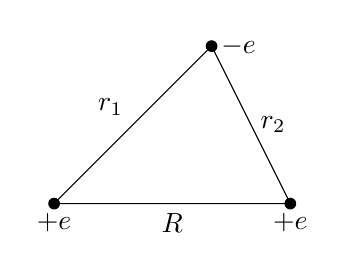
\begin{tikzpicture} \draw[] (0,0) node[below]{$+e$} node[circle, fill=black,inner sep=1.5pt]{} -- (3,0) node[pos=0.5, below]{$R$} node[below]{$+e$} node[circle, fill=black,inner sep=1.5pt]{} -- (2,2) node[pos=0.5, right]{$r_2$} node[right]{$-e$} node[circle, fill=black,inner sep=1.5pt]{} -- (0,0) node[pos=0.5, above left]{$r_1$};
\end{tikzpicture} 
\caption{ہائیڈروجن سالمہ بارداریہ، \عددی{\ce{H}_2^+}} 
\label{شکل_تغیریت_ہائیڈروجن_سالمہ_بارداریہ} 
\end{figure} 

 آزمائشی تفاعل موج تیار کرنے کی خاطر فرض کریں کہ  زمینی حال  (مساوات \حوالہ{مساوات_تین_ابعاد_زمینی_ہائیڈروجن})
\begin{align}
\psi_{0}(\kvec{r})=\frac{1}{\sqrt{\pi a^{3}}}e^{-r/a} 
\end{align}
  میں  ہائیڈروجن جوہر کے قریب  فاصلہ \عددی{ R} پر ،   دوسرا پروٹان "    لا متناہی" سے  لا کر رکھتے ہوئے   بارداریہ پیدا کیا جاتا ہے۔ اگر رداس بوہر سے \عددی{R} کافی زیادہ  ہو تب الیکٹران کا تفاعل موج غالباً زیادہ تبدیل نہیں ہو گا۔ تاہم ہم دونوں پروٹان کو ایک نظر سے دیکھنا  چاہیں گے،  لہٰذا دونوں  کے ساتھ الیکٹران کی وابستگی کا احتمال ایک  جیسا ہوگا۔ یوں ہم آمادہ ہوتے ہیں  کہ  درجہ ذیل روپ کا آزمائشی تفاعل استعمال کریں۔ 
 \begin{align}
\psi=A[\psi_{0}(r_{1})+\psi_{0}(r_{2})]
\end{align}
(چونکہ ہم سالماتی    تفاعل موج کو جوہری مدارچوں کا خطی جوڑ لکھتے ہیں لہٰذا ماہر کوانٹائی  کیمیا اس  کو \اصطلاح{ جوہری مدارچوں کی خطی جوڑ   ترکیب}\فرہنگ{جوہری مدارچوں!  خطی جوڑ ترکیب}\حاشیہب{LCAO technique}\فرہنگ{LCAO} کہتے ہیں۔ )

پہلا کام  آزمائشی تفاعل کی معمول زنی ہے۔
 \begin{multline}\label{مساوات_تغیریت_معمول_زنی}
1=\int\abs{\psi}^{2}\dif^{\,3}\kvec{r}=\abs{A}^{2}\big [\int \abs{\psi_{0}(r_{1})}^{2} \dif^{\,3}\kvec{r}\\
+\int \abs{\psi_{0}(r_{2})}^{2}\dif^{\,3}\kvec{r}+2\int\psi_{0}(r_{1})\psi_{0}(r_{2})\dif^{\,3}\kvec{r}\big ]
\end{multline}
 پہلے دو تکملات  \عددی{1}ہیں ( چونکہ  \عددی{\psi_{0}} معمول شدہ ہے)؛ تیسرا زیادہ پیچیدہ ہے۔ درجہ ذیل لیں۔
 \begin{align}\label{مساوات_تغیریت_پیچیدہ_لیں}
I\equiv\langle \psi_{0}(r_{1})|\psi_{0}(r_{2})\rangle=\frac{1}{\pi a^{3}}\int e^{-(r_{1}+r_{2})/a}\dif^{\,3}\kvec{r}
\end{align}
 ایسا محددی  نظام کھڑا کر کے،  جس کے  مبدا  پر پروٹان \عددی{ 1} اور  \عددی{z}  محور پر  \عددی{ R} فاصلے   پر پروٹان  \عددی{2 }  ہو (شکل \حوالہ{شکل_تغیریت_محدد_قدار_آئے})، 
\begin{align}
r_{1}=r \quad \text{\RL{اور}}\quad r_{2}=\sqrt{r^{2}+R^{2}-2rR\cos{\theta}} 
\end{align}
 %
\begin{figure} 
\centering
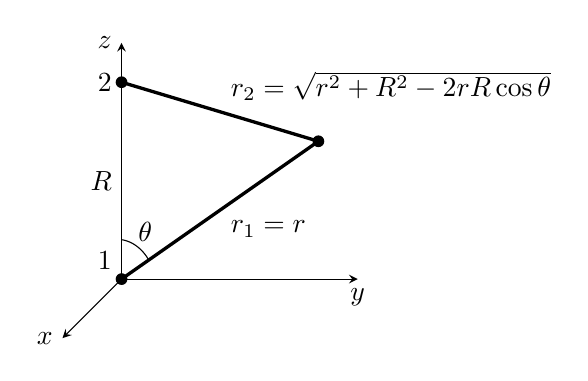
\begin{tikzpicture}[x={(-0.5cm,-0.5cm)}, y={(1cm,0cm)}, z={(0cm,1cm)}]
\pgfmathsetmacro{\p}{atan(2/0.5)} \pgfmathsetmacro{\t}{acos(2/sqrt(0.5^2+2.75^2+2^2))} \draw[-stealth] (0,0,0) -- (1.5,0,0) node[left]{$x$};
\draw[-stealth] (0,0,0) -- (0,3,0) node[below]{$y$};
\draw[-stealth] (0,0,0) -- (0,0,3) node[left]{$z$};
\draw[] (0,0,0) node[above left]{$1$} node[circle, fill=black,inner sep=1.5pt]{} -- (0,0,2.5) node[left]{$2$} node[pos=0.5,left]{$R$};
\draw[very thick] (0,0,2.5) node[circle, fill=black,inner sep=1.5pt]{} -- (0.5, 2.75, 2) node[pos=0.5,above right]{$r_2=\sqrt{r^2 + R^2 -2rR\cos \theta}$} node[circle, fill=black,inner sep=1.5pt]{};
\draw[very thick] (0,0,0) -- (0.5,2.75,2) node[pos=0.5,below right]{$r_1=r$};
\draw[domain=0:\t] plot ({0.5*sin(\x)*cos(\p)},{0.5*sin(\x)*sin(\p)},{0.5*cos(\x)});
\draw(0,0.3,0.6)node[]{$\theta$};
\end{tikzpicture} 
\caption{مقدار \عددی{I} کے حساب کی خاطر محدد (مساوات \حوالہ{مساوات_تغیریت_پیچیدہ_لیں})۔} 
\label{شکل_تغیریت_محدد_قدار_آئے} 
\end{figure} 
%
ہوں گے لہٰذا درجہ ہوگا ۔
\begin{align}
I=\frac{1}{\pi a^{3}}\int e^{-r/a}e^{-\tfrac{\sqrt{r^{2}+R^{2}-2rR\cos{\theta}}}{a}}\,r^{2}\sin{\theta}\dif r\dif \theta \dif \phi
\end{align}
 متغیر  \عددی{\phi}  کا (نہایت آسان) تکمل   \عددی{2\pi}  دے گا۔ متغیر   \عددی{\theta}   کا تکمل  کرنے کی خاطر درجہ ذیل لیں۔
\begin{align*}
y\equiv\sqrt{r^{2}+R^{2}-2rR\cos{\theta}}\quad  \Rightarrow \quad \dif (y^{2})=2y\dif y=2rR\sin{\theta}\dif \theta
\end{align*}
  تب درجہ ذیل ہوگا۔
\begin{multline*}
\int_{0}^{\pi}e^{-\tfrac{\sqrt{r^{2}+R^{2}-2rR\cos{\theta}}}{a}}\sin{\theta}\dif \theta=\frac{1}{rR}\int_{\abs{r-R}}^{r+R}e^{-y/a}y\dif y\\
=-\frac{a}{rR}\big[e^{-(r+R)/a}(r+R+a)-e^{-\abs{r-R}/a}(\abs{r-R}+a)\big]
\end{multline*}
 اب تکمل \عددی{ r}  با آسانی حل ہوگا۔ 
\begin{multline*}
I=\frac{2}{a^{2}R}\big[-e^{-R/a}\int_{0}^{\infty}(r+R+a)e^{-2r/a}r\dif r+e^{-R/a}\int_{0}^{R}(R-r+a)r\dif r\\
+e^{R/a}\int_{R}^{\infty}(r-R+a)e^{-2r/a}r\dif r\big]
\end{multline*}
 ان تکملات کی قیمتوں کے حساب   کے بعد   الجبرائی   تسہیل  سے  درجہ ذیل حاصل ہوگا۔
\begin{align}
I=e^{-R/a}\big[1+\big(\frac{R}{a}\big)+\frac{1}{3}\big(\frac{R}{a}\big)^{2}\big]
\end{align}
ہم \عددی{I}   کو    \اصطلاح{ڈھانپائی تکمل}\فرہنگ{تکمل!ڈھانپائی}\حاشیہب{overlap integral}\فرہنگ{overlap integral}  کہتے ہیں؛  جو \عددی{\psi_{0}(r_{1})}  کے    \عددی{\psi_{0}(r_{2}}  پر چڑھنے کی مقدار کی پیمائش ہے ( دھیان رہے کہ   \عددی{R\rightarrow 0}  کی صورت میں یہ \عددی{1} کو ،  اور    \عددی{R\rightarrow \infty}   کی صورت  \عددی{0} کو پہنچتا ہے)ڈھانپائی تکمل \عددی{I} کی صورت    میں مستقل   معمول زنی   (مساوات  \حوالہ{مساوات_تغیریت_معمول_زنی})درجہ ذیل ہوگا ۔
\begin{align}
\abs{A}^{2}=\frac{1}{2(1+I)} 
\end{align}

 اس کے بعد ہمیں آزمائشی حال  \عددی{\psi}  میں \عددی{H} کی توقعاتی قیمت کا حساب کرنا ہوگا۔ یاد رہے کہ 
 \begin{align*}
\big(-\frac{\hslash^{2}}{2m}\nabla^{2}-\frac{e^{2}}{4\pi\epsilon_{0}}\frac{1}{r_{1}}\big)\psi_{0}(r_{1})=E_{1}\psi_{0}(r_{1})
\end{align*}
ہو گا (  جہاں   \عددی{E_{1}=\SI{-13.6}{\electronvolt}}  جوہری ہائیڈروجن کی زمینی حال توانائی ہے)؛  اور \عددی{r_1} کی جگہ \عددی{ r_2} کے لئے بھی ایسا ہی   ہو گا؛ لہٰذا  درجہ ذیل ہوگا ۔
\begin{align*}
 H\psi&=A\big[-\frac{\hslash^{2}}{2m}\nabla^{2}-\frac{e^{2}}{4\pi\epsilon_{0}}\big(\frac{1}{r_{1}}+\frac{1}{r_{2}}\big)\big][\psi_{0}(r_{1})+\psi_{0}(r_{2})]\\
&=E_{1}\psi-A\big(\frac{e^{2}}{4\pi\epsilon_{0}}\big)\big[\frac{1}{r^{2}}\psi_{0}(r_{1})+\frac{1}{r_{1}}\psi_{0}(r_{2})\big]
\end{align*}
 یوں\عددی{ H} کی توقعاتی قیمت درجہ ذیل ہوگی۔
\begin{align}
\langle H \rangle =E_{1}-2\abs{A}^{2}\big(\frac{e^{2}}{4\pi\epsilon_{0}}\big)\big[\langle \psi_{0}(r_{1})\abs{\frac{1}{r_{2}}}\psi_{0}(r_{1})\rangle +\langle \psi_{0}(r_{1})\abs{\frac{1}{r_{1}}}\psi_{0}(r_{2})\rangle\big]
\end{align}
 میں آپ کے لئے باقی دو مقدار جو\اصطلاح{ بلا واسطہ تکمل}:\فرہنگ{بلاواسطہ تکمل}\حاشیہب{direct integral}\فرہنگ{direct integral} 
\begin{align}
D\equiv a\langle \psi_{0}(r_{1})\abs{\frac{1}{r_{2}}}\psi_{0}(r_{1})\rangle
\end{align}
 اور  \اصطلاح{مبادلہ تکمل}:\فرہنگ{مبادلہ تکمل}\حاشیہب{exchange integral}\فرہنگ{exchange integral} 
\begin{align}
X\equiv a\langle\psi_{0}(r_{1})\abs{\frac{1}{r_{1}}}\psi_{0}(r_{2})\rangle
\end{align}
 کہلاتے ہیں،  حل کرنے کے لئے چھوڑتا ہوں۔ بلا واسطہ تکمل کا نتیجہ:
\begin{align}
D=\frac{a}{R}-\big(1+\frac{a}{R}\big)e^{-2R/a} 
\end{align}
 اور مبادلہ تکمل کا نتیجہ درجہ ذیل ہے  (سوال \حوالہ{سوال_تغیریت_بلاواسطہ_معادل_تکملات} دیکھیں)۔  
\begin{align}
X=\big(1+\frac{R}{a}\big)e^{-R/a} 
\end{align}

 ان تمام نتائج کو اکٹھے کرتے ہوئے اور ( مساوات \حوالہ{مساوات_ابعادی_ہائیڈروجن_اجازتی_توانائیاں}  اور مساوات \حوالہ{مساوات_تین_ابعادی_رداس_بوہر}  کو)  یاد  کرتے
   ہوئے کہ  \عددی{E_{1}=-\tfrac{e^{2}}{4\pi\epsilon_{0}}\tfrac{1}{2a}} ہے،ہم درجہ ذیل اخذ کرتے ہیں۔
\begin{align}
\langle H \rangle =\big[1+2\frac{(D+X)}{(1+I)}\big]E_{1} 
\end{align}
 اصول تغیریت کے تحت،   زمینی حال توانائی  \عددی{\langle H \rangle}  سے کم ہو  گی۔ یقیناً،  یہ صرف الیکٹران کی توانائی ہے؛ اس کے علاوہ  پروٹان پروٹان دفع سے وابستہ مخفی توانائی:
\begin{align}
V_{pp}=\frac{e^{2}}{4\pi\epsilon_{0}}\frac{1}{R}=-\frac{2a}{R}E_{1} 
\end{align}
 بھی پائی جاتی ہے۔  یوں نظام کی  \ترچھا{کل}  توانائی   ( \عددی{-E_{1}}  کی اکائیوں میں)،     \عددی{x\equiv R/a}  کا تفاعل لکھتے ہوئے،  درجہ ذیل سے کم ہو گی۔
 \begin{align}\label{مساوات_تغیریت_کل_توانائی_اس_سے_کم}
F(x)=-1+\frac{2}{x}\Big\{\frac{(1-(2/3)x^{2})e^{-x}+(1+x)e^{-2x}}{1+(1+x+(1/3)x^{2})e^{-x}}\Big\} 
\end{align}
 اس تفاعل کو شکل  \حوالہ{شکل_تغیریت_مقید_حال} میں ترسیم کیا گیا ہے۔ اس ترسیم کا کچھ حصہ \عددی{-1} سے نیچے ہے،  جہاں معادل جوہر جمع ایک آزاد پروٹان کی 
 توانائی \عددی{(\SI{-13.6}{\electronvolt})} سے  کم ہے،  لہٰذا اس نظام میں بندھ پیدا ہوگا۔ یہ ایک شریک گرفتی بندھ  ہوگا، جہاں الیکٹران  دونوں پروٹان کا   برابر شریک  ہوگا۔ پروٹان کے بیچ   توازنی فاصلہ تقریباً \عددی{2.4}  رداس بوہر،  یعنی \عددی{\SI{0.13}{\nano\meter}}    ہے ( تجرباتی قیمت  \عددی{\SI{0.106}{\nano\meter}} ہے)۔بندشی  توانائی  کے  حساب سے حاصل قیمت  \عددی{\SI{1.8}{\electronvolt}}،  جبکہ پیمائشی قیمت  \عددی{\SI{2.8}{\electronvolt}} ہے (  اصول تغیریت ہمیشہ زمینی حال توانائی سے تجاوز کرتا ہے،  لہٰذا یہ طاقت بندھ  کی کم  قیمت  دے گا؛  بہرحال اس کی فکر نہ کریں:)  یہاں اہم نقطہ یہ  ہے کہ بندھ  پایا جاتا ہے؛  بہتر  تغیری  تفاعل اس مخفیہ کو مزید گہرا بنائے  گا۔
\begin{figure} \centering
\begin{tikzpicture}[declare function={fa(\x)=(1-2/3*\x^2)*e^(-\x); fb(\x)=(1+\x)*e^(-2*\x); fc(\x)=1+(1+\x+1/3*\x^2)*e^(-\x); f(\x)=-1+2*(fa(\x)+fb(\x))/(\x*fc(\x));}]
\begin{axis}[axis lines=middle,axis x line shift=1,xlabel={$x$},ylabel={$F(x)$}, xtick={1,2,2.25,3,4,5,6}, xticklabels={$1$,$2$,,$3$,$4$,$5$,$6$}, ytick={-1.2,-1,-0.5,0}, ylabel style={at={(current axis.above origin)},anchor=east},,enlargelimits,ymax=0,ymin=-1.3]
\addplot [thick,domain=0.7:6,smooth] {f(x)};
\addplot[thick] coordinates {(2.25,-1.025)(2.25,-0.975)};
\addplot[] coordinates{(2.25,-1)} node[pin={45:{توازن}}]{};
\end{axis} \end{tikzpicture} 
\caption{تفاعل \عددی{F(x)} (مساوات \حوالہ{مساوات_تغیریت_کل_توانائی_اس_سے_کم}) کی ترسیم مقید حال کی موجودگی دکھاتی ہے (بوہر رداس کی اکائیوں میں \عددی{x} دو پروٹان کے بیچ فاصلہ ہے)۔ } 
\label{شکل_تغیریت_مقید_حال} 
\end{figure} 

 %KKK edited till here 28 jan 2022
 
\ابتدا{سوال}\شناخت{سوال_تغیریت_بلاواسطہ_معادل_تکملات}
 % 
7.8\\
بلاواسطہ تکمل D اور مبادلہ تکمل X مساوات 7.45 اور 7.46 کی قیمتیں تلاش کریں۔ اپنے جوابات کا موازنہ مساوات 7.47 اور 7.48 کے ساتھ کریں۔ 
\انتہا{سوال}
\ابتدا{سوال}
 % 
7.9\\
فرض کریں ہم نے پھرکی تفاعل موج مساوات 7.37 میں منفی علامت استعمال کی ہوتی ۔
\begin{align}
\psi=A[\psi_{0}(r_{1})-\psi_{0}(r_{2})]
\end{align}
 کوئی نیا تکمل حل کیے بغیر مساوات 7.51 کا مماثل \عددی{ F(x)} معلوم کر کے ترسیم کریں۔ دکھائیں کہ ایسی صورت میں بند پیدا نہیں ہوگا۔ چونکہ اصول تغیریت صرف بالائی حد بندی دیتا ہے لہٰذا اس سے یہ ثابت نہیں ہوگا کہ ایسے حال میں بند نہیں پایا جائے گا۔ تاہم اس سے زیادہ امید بھی نہیں کرنی چاہیے۔ تبصرہ در حقیقت درجہ ذیل روپ کا کوئی تفاعل 
\begin{align}
\psi=A[\psi_{0}(r_{1})+e^{i\phi}\psi_{0}(r_{2})]
\end{align}
 کی ایک خاصیت یہ ہے کہ الیکٹران دونوں پروٹان کے ساتھ برابر کا وابستگی رکھتا ہے۔ تاہم چونکہ باہمی ادل بدل  \عددی{P: r_{1}\leftrightarrow r_{2}} کی صورت میں ہیملٹنی مساوات 7.35 غیر متغیر ہے۔ لہٰذا اس کے امتیازی تفاعلات کو بیک وقت P کے امتیازی تفاعلات چنا جا سکتا ہے۔ امتیازی قدر \عددی{+1} کے ساتھ مثبت علامت۔ مساوات 7.37 اور امتیازی قدر منفی 1 کے ساتھ منفی علامت مساوات 7.52 ہوگا۔ زیادہ عمومی صورت مساوات 7.53 کا استعمال مزید فائدہ نہیں دے گا۔ اگرچہ آپ چاہیں تو اسے استعمال کر کے دیکھ سکتے ہیں۔
 \انتہا{سوال}
\ابتدا{سوال}
 % 
7.10\\
نقطہ توازن پر \عددی{ F(x)}  کی دوہرا تفرق سے ہائیڈروجن سالمہ بارداریہ حصہ 2.3 میں دونوں پروٹان کی ارتعاش کی قدرتی تعدد اومیگہ کی انداز قیمت تلاش کی جا سکتی ہے۔ اگر اس موردیش کی زمینی حال توانائی   \عددی{\hslash\omega/2}  نظام کی بندشی توانائی سے زیادہ ہو تب نظام بکھر کر ٹوٹ جائے گا ۔ دکھائیں کہ حقیقت میں موردیش توانائی اتنی کم ہے کہ ایسا کبھی بھی نہیں ہوگا۔ ساتھ ہی مقید لرزشی سطحوں کی انداز تعداد دریافت کریں۔ تبصرہ 
آپ دہلیلی طور پر کم سے کم نقطہ یا اس نقطہ پر دوہرا تفرق حاصل نہیں کر پائیں گے۔ اعدادی طریقہ یا کمپیوٹر کی مدد سے ایسا کیجئے گا۔
\انتہا{سوال}
\ابتدا{سوال}
 % 
7.11\\
الف ) درج ذیل روپ کا برقی تفاعل موج
\begin{align}
\psi(x)=\begin{cases} A\cos{(\pi x/a)} & (-a/2<x<a/2)\\
0\\
\end{cases} 
\end{align}
 دیگر صورت
اس کا استعمال کرتے ہوئے یک بُعدی ہارمونی مرتعش کی زمینی حال توانائی کی حد بندی تلاش کریں ۔ a کی بہترین قیمت کیا ہوگی ۔ H کمتر کا موازنہ ٹھیک توانائی سے کریں ۔
تبصرہ : برقی تفاعل میں \عددی{\pm a/2} پر ایک بل پایا جاتا ہے ایک غیر استمراری تفرق کیا آپ تو اس سے نمٹنا ہوگا جیسے مجھے مثال 7.3 میں نمٹنا پڑا۔
ب ) وقفہ \عددی{\psi(x)=B\sin{(\pi x/a)}} پر \عددی{(-a,a)} استعمال آتے ہوئے پہلے حال کی حد بندی تلاش کریں ۔ اپنے جواب کا ٹھیک ٹھیک جواب کے ساتھ موازنہ کریں ۔
\انتہا{سوال}
\ابتدا{سوال}
 % 
7.12\\
الف ) درج ذیل برقی تفاعل موج 
\begin{align}
\psi(x)=\frac{A}{(x^{2}+b^{2})^n} 
\end{align}
 جہاں n اختیاری مستقل ہے استعمال کرتے ہونے سوال 7.2 کو عمومیت دیں مقدار معلوم b کی بہترین قیمت درج ذیل دے گا۔
\begin{align}
b^{2}=\frac{\hslash}{m\omega}\big[\frac{n(4n-1)(4n-3)}{2(2n+1)}\big]^{1/2} 
\end{align}
 ب ) ہارمونی مرتعش کی پہلی ہیجان حال تو بالائی حد بندی کی کم سے کم قیمت درج ذیل برقی تفاعل استعمال کرتے ہوئے معلوم کریں ۔
\begin{align}
\psi(x)=\frac{Bx}{(x^{2}+b^{2})^n} 
\end{align}
 جزوی جواب مقدار معلوم b کی بہترین قیمت درج ذیل دے گا ۔
\begin{align}
b^{2}=\frac{\hslash}{m\omega}\big[\frac{n(4n-5)(4n-3)}{2(2n+1)}\big]^{1/2} 
\end{align}
 ج ) آپ دیکھیں گے کہ \عددی{ n\rightarrow \infty} حد بندی بالکل ٹھیک توانائیوں تک پہنچتی ہے ۔ ایسا کیوں ہے ؟
اشاره : برقی تفاعلات امواج کو \عددی{n=2,n=3} اور \عددی{n=4} کے لیے ترسیم کرتے ہوئے ان کا موازنہ اصل تفاعلات موج مساوات 2.59اور 2.62 کے ساتھ کریں ۔ تحلیلی طور پر ایسا کرنے کی خاطر درج ذیل مماثل سے آغاز کریں ۔
\begin{align}
e^{z}=\lim_{n \to \infty}(1+\frac{z}{n})^{n} 
\end{align}
\انتہا{سوال}
 \ابتدا{سوال}
 % 
1.13\\
ہائیڈروجن کی زمینی حال کی کم سے کم حد بندی گاوسی برقی موج تفاعل
\begin{align}
\psi(r)=Ae^{-br^{2}} 
\end{align}
 استعمال کرتے ہوئے تلاش کریں ۔ جہاں معمول زنی سے A تعین ہوگا جبکہ b قابل تبدیل مقدار معلوم ہے ۔ جواب \عددی{-11.5\text{eV}}
 \انتہا{سوال}
\ابتدا{سوال}
 % 
7.14\\
اگر نوریہ کی کمیت غیر صفر \عددی{(m_{\gamma}\neq 0)} ہوتی تب مخفیہ کی جگہ یو کوا مخقیا
\begin{align}
V(r)=\frac{-e^{2}}{3\pi\epsilon_{0}}\frac{e^{-\mu r}}{r} 
\end{align}
 استعمال ہوتا جہاں \عددی{(\mu=m_{\gamma}c/\hslash)} ہے ۔ اپنی مرضی کا برقی تفاعل موج استعمال کرتے ہوئے اس مخفیہ کے ہائیڈروجن  جوہر کی بندشی توانائی کی قیمت معلوم کریں ۔ آپ \عددی{\mu a <<1} لیں اور اپنے جواب کو \عددی{(\mu a)^{2}} رتبی درستگی تک لکھیں۔
 \انتہا{سوال}
\ابتدا{سوال}
 % 7.15
فرض کریں آپکو ایک ایسا کوانٹائی نظام دیا جاتا ہے جس کا ہیملٹنی \عددی{H_{0}} صرف دو امتیازی حالات کا حامل ہو \عددی{\psi_{a}} جس کی توانائی \عددی{E_{a}} اور \عددی{\psi_{b}} جس کی توانائی \عددی{E_{b}} ہو ۔ یہ عموری معمول شدہ اور غیر انہتا تی ہے ۔ مزید فرض کریں کہ \عددی{E_{a}<E_{b}} ہے ۔ اب ہم اضطراب \عددی{H'} چالو کرتے ہیں ۔ جس کے قالبی ارکان درج ذیل ہیں ۔
\begin{align}
\langle \psi_{a}|H'|\psi{a}\rangle=\langle \psi_{b}|H'|\psi{b}\rangle=0\quad \langle \psi_{a}|H'|\psi{b}\rangle=\langle \psi_{b}|H'|\psi{a}\rangle=h
\end{align}
 جہاں h کوئی مخصوص مستقل ہے۔
الف ) مضطرب ہیملٹنی کی امتیازی اقدار کی ٹھیک ٹھیک قیمتیں تلاش کریں ۔
ب ) رتبہ دوم نظریہ اضطراب استعمال کرتے ہوئے مضطرب نظام کی توانائیوں کی انداز ی قیمت معلوم کریں ۔
ج ) مضطرب نظام کی زمینی حال کی توانائی کی اندازی قیمت درج ذیل روپ کا برقی تفاعل
\begin{align}
\psi=(\cos{\phi})\psi_{a}+(\sin{\phi})\psi_{b} 
\end{align}
 استعمال کر کہ اصول تغیریت سے حاصل کریں ۔ جہاں \عددی{\phi} قابل تبدیل مقدار معلوم ہے ۔
تبصرہ : اضطراب کا خطی جوڑ لازماً معمول شدہ دے گا۔
د ) اپنے جوابات کا جزو الف ، ب ، اور ج کے ساتھ موازنہ کریں ۔ یہاں اصول تغیریت اتنا زیادہ درست کیوں ہے ؟
\انتہا{سوال}
\ابتدا{سوال}
 % 7۔16
ہم سوال 7۔15 میں تیار کی گئی ترکیب مثال کے طور پر یکساں مقناطیسی میدان \عددی{\kvec{B}=B_{z}\hat{k}} میں ایک ساکن الیکٹران پر غور کرتے ہیں ۔ جس کا ہیملٹنی مساوات 4۔158 درج ذیل ہوگا
\begin{align}
H_{0}=\frac{eB_{z}}{m}S_{z} 
\end{align}
 امتیازی چکر کار \عددی{x_{a}} اور \عددی{x_{b}} ان کی مطابقتی توانائیاں \عددی{E_{a}} اور \عددی{E_{b}} مساوات 7.161 میں دی گئی ہیں ۔
اب ہم X رخ درج ذیل روپ کے یکساں میدان
\begin{align}
H'=\frac{eB_{x}}{m}S_{x} 
\end{align}
 کے اضطراب کو چالو کرتے ہیں ۔
الف ) اضطراب \عددی{H'} کے قالبی ارکان تلاش کر کہ تصدیق کریں کہ ان کا ساخت مساوات 7.55 تو طرح ہے یہاں H کیا ہوگا ؟
ب ) دوم رتبی نظریہ اضطراب میں نئی زمینی حال تونائی کو سوال 7.15 ( ب ) استعمال کرتے ہوئے تلاش کریں ۔
ج ) زمینی حال توانائی کی حد بندی سوال 7.15 ( ج ) کا نتیجہ استعمال کرتے ہوئے اصول تغیریت سے حاصل کریں
\انتہا{سوال}
\ابتدا{سوال}\شناخت{سوال_تغیریتی_ہیلیم_نما_غیر_کولمب}
 % 
7.17\\
اگرچہ ہیلیم کے لیے مساوات شروڈنگر کو ٹھیک ٹھیک حل نہیں کیا جا سکتا ہے مگر بیلیم کے ایسے نظام پائے جاتے ہیں جن کے ٹھیک ٹھیک حل معلوم کیے جا سکتے ہیں ۔ اس کی ایک  سادہ مثال ربڑی پٹی بیلیم ہے جس میں کو توں کی بجائے قانون ہک کی درج ذیل قوتیں استعمال ہونگی
\begin{align}
H=\frac{-\hslash^{2}}{2m}(\nabla_{1}^{2}+\nabla_{2}^{2})+\frac{1}{2}m\omega^{2}(r_{1}^{2}+r_{2}^{2})-\frac{\lambda}{4}m\omega^{2}\abs{\kvec{r_{1}}-\kvec{r_{2}}}^{2} 
\end{align}
 الف ) دکھائیں کہ متغیرات \عددی{\kvec{r_{1}}, \kvec{r_{2}}} کی بجائے متغیرات
\begin{align}
\kvec{u}\equiv\frac{1}{\sqrt{2}}(\kvec{r_{1}}+\kvec{r_{2}})\quad \kvec{v}\equiv\frac{1}{\sqrt{2}}(\kvec{r_{1}}-\kvec{r_{2}})
\end{align}
 استعمال کرنے سے ہیملٹنی دو علیحدہ علیحدہ تین آبادی ہارمونی  مرتعشات میں تقسیم ہوگا۔
\begin{align}
H=[\frac{-\hslash^{2}}{2m}\nabla_{\mu}^{2}+\frac{1}{2}m\omega^{2}\mu^{2}]+[\frac{-\hslash^{2}}{2m}\nabla_{\nu}^{2}+\frac{1}{2}(1-\lambda)m\omega^{2}\nu^{2}]
\end{align}
 ب ) اس نظام کی ٹھیک ٹھیک زمینی حال توانائی کیا ہوگی ؟
ج ) ٹھیک ٹھیک حل نہ جاننے تو صورت میں ہم ہیملٹنی کی اصل صورت مساوات 7.59 پر حصہ 7.2 کی ترکیب استعمال کرنا چاہیں گے۔
سپر کرنے کو نظر انداز کرتے ہوئے حساب کیجیے گا ۔ اپنے جواب کا ٹھیک ٹھیک جواب کے ساتھ موازنہ کریں ۔
جواب: \عددی{\langle H \rangle =3\hslash\omega(1-\lambda/4)}
\انتہا{سوال}
\ابتدا{سوال}
 % 
7.18\\
ہم نے سوال 7.7 میں دیکھا کہ سپرشدہ برقی تفاعل موج ، مساوات 7.27 جو بیلیم کے لیے مفید ثابت ہوا منفی ہائیڈروجن بارداریہ میں مقید حال میں موجودگی کی تصدیق کرنے کے لیے کافی نہیں ہے ۔ چندرشیكر  نے درج ذیل کا برقی تفاعل موج استعمال کیا
\begin{align}
\psi(\kvec{r_{1}},\kvec{r_{2}})\equiv A[\psi_{1}(r_{1})\psi_{2}(r_{2})+\psi_{2}(r_{1})\psi_{1}(r_{2})]
\end{align}
 جہاں درج ذیل ہے
\begin{align}
\psi_{1}(r)\equiv \sqrt{\frac{z_{1}^{3}}{\pi a^{3}}}e^{-z_{1}r/a} \quad \psi_{2}(r)\equiv \sqrt{\frac{z_{2}^{3}}{\pi a^{3}}}e^{-z_{2}r/a} 
\end{align}
 
یعنی انہوں نے دو مختلف سپر اجزائے ضربی کی اجازت دی ایک الیکٹران کو مرکزہ کے قریب اور دوسرے کو مرکزہ سے دور تصور کیا گیا۔ چونکہ الیکٹران متماثل ذرہ ہے لہٰذا فضائی تفاعل موج کو باہمی مبادلہ کے لحاظ سے لازماً تشاکلی بنانا ہوگا چکر حال جس کا موجودہ حساب میں کوئی کردار نہیں پایا جاتا خلاف تشاکلی ہے ۔ دکھائیں کہ قابل تبدیل مقدار معلوم \عددی{Z_{1}} اور \عددی{Z_{2}} کی قیمتوں کو سوچ کہ منتخب کرنے سے \عددی{\langle H \rangle } کی قیمت \عددی{-13.6\text{eV}} سے کم حاصل کی جا سکتی ہے ۔
جواب:
\begin{align}
\langle H \rangle = \frac{E_{1}}{x^{6}+y^{6}}(-x^{8}+2x^{7}+\frac{1}{2}x^{6}y^{2}-\frac{1}{2}x^{5}y^{2}-\frac{1}{8}x^{3}y^{4}+\frac{11}{8}xy^{6}-\frac{1}{2}y^{8})
\end{align}
 جہاں \عددی{x\equiv Z_{1}+Z_{2}z} اور \عددی{y\equiv2\sqrt{Z_{1}Z_{2}}} ہیں ۔ چندر شیکر نے \عددی{Z_{1}=1.039} چونکہ یہ ایک سے بڑا ہے لہٰذا اس کو موثر مرکزی بار تصور نہیں کیا جا سکتا ہے ۔ تاہم اس کے باوجود اس کو برقی تفاعل موج قبول کیا جا سکتا ہے ۔ اور \عددی{Z_{2}=0.283} استعمال کیا
 \انتہا{سوال}
\ابتدا{سوال}
 % 
7۔19\\
جوبری برکن کو برقرار رکھنے میں بنیادی مسئلہ دو ذرات مثلاً دو ڈیوٹران کو ایک دوسرے کے اتنا قریب لانا ہے کہ کولمب قوت دفع پر ان کے بیچ کششی تاہم اثر قریب مرکزی قوتیں سبقت لے جائیں ہم ذرات کو شاندار درجہ حرارت تک گرم کر کہ ان کو بلا منصوبہ  تصادم کے ذریعے انہیں ایک دوسرے کے قریب زبردستی لا سکتے  ہیں ۔ دوسری تجویز میون عمل انگیز کا استعمال ہے جس میں ہم ہائیڈروجن سالمہ باردا پراٹان کی جگہ ڈیوٹران اور الیکٹران کی جگہ میون رکھ کر تیار کرتے ہیں ۔ اس ساخت میں ڈیوٹران کے بیچ توازنی فاصلہ کی پیش گوئی کریں   اور سمجھائیں کہ اس مقصد کی خاطر کیوں الیکٹران سے میون بہتر ثابت ہوگا۔
\انتہا{سوال}
\ابتدا{سوال}\شناخت{سوال_تغیریتی_نفیس_آزمائشی_تفاعل}
 % 
7.20\\
کوانٹائی نقطے فرض کریں ایک ذرہ تو شکل \حوالہ{شکل_تغیریت_صلیبی_خطہ} میں دکھائے گئے سلیبی خطہ پر دو ابعاد میں حرکت کرنے کا پابند بنایا جائے سلیبی ہاتھ لامتناہی تک پہنچتے ہیں . سلیب کے اندر مخفیہ صفر ہے جو کہ اس کے بایر لامتناہی ہے ۔ حیرانی کی بات ہے کہ یہ تشکیل مثبت توانائی مقید حال کا حامی ہے۔

\begin{figure} \centering
\begin{tikzpicture} \draw[-stealth] (-3,0) -- (3.25,0) node[below]{$x$};
\draw[-stealth] (0,-2) -- (0,2.25) node[left]{$y$};
\fill[,color=lgray] (-3,-1) rectangle (-1,-2);
\fill[,color=lgray] (-3,1) rectangle (-1,2);
\fill[,color=lgray] (3,-1) rectangle (1,-2);
\fill[,color=lgray] (3,1) rectangle (1,2);
\draw[thick] (-3,-1) -- (-1,-1) -- (-1,-2);
\draw[thick] (-3,+1) -- (-1,+1) -- (-1,+2);
\draw[thick] (3,-1) -- (1,-1) -- (1,-2);
\draw[thick] (3,1) -- (1,1) -- (1,2);
\draw[](-0.1,1) -- (0.1,1) node[right]{$a$};
\draw[](-0.1,-1) -- (0.1,-1) node[right]{$-a$};
\draw[](-1,0.1) -- (-1,-0.1) node[below]{$-a$};
\draw[](1,0.1) -- (1,-0.1) node[below]{$a$};
\end{tikzpicture} 
\caption{صلیبی خطہ برائے سوال \حوالہء{7.20}} 
\label{شکل_تغیریت_صلیبی_خطہ} 
\end{figure} 
الف ) دکھائیں کہ کم سے کم توانائی جو لامتناہی تک پہنچتی ہے درج ذیل ہے
\begin{align}
E_{\text{threshold}}=\frac{\pi^{2}\hslash^{2}}{8ma^{2}};
\end{align}
 اس سے کم توانائی کا ہر حل لامتناہی کا مقید ہوگا۔
اشاره : ایک بازو پر \عددی{(x>>a)} مساوات شروڈنگر کو علیحدگی متغیرات کو مدد سے حل کریں ۔ اگر تفاعل موج لامتناہی تک پہنچتی ہے تب اس کا x پر انحصار \عددی{e^{ik_{x}x}} جہاں \عددی{k_{x}>0} ہے کو روپ میں ہوگا۔
ب ) اب اصول تغیریت استعمال کرتے ہوئے دکھائیں کہ  E سے کم توانائی زمینی حال کا ہوگا۔ درج ذیل برقی تفاعل موج استعمال کریں 
\begin{align}
\psi(x.y)=A\begin{cases} (1-\abs{xy}/a^{2})e^{-\alpha} & \abs{x}\leq a,\abs{y}\leq a\\
(1-\abs{x}/a)e^{-\alpha\abs{y}/a} & \abs{x}\leq a ,\abs{y}> a\\
(1-\abs{y}/a)e^{-\alpha\abs{x}/a} & \abs{x}> a,\abs{y}\leq a\\
0\\
\end{cases} 
\end{align}
 اس کی  معمول زنی کرکے  A تعین کریں ۔ اور H کی توقعاتی قیمت کا حساب لگائیں۔
جواب :
\begin{align}
\langle H \rangle=\frac{3\hslash^{2}}{ma^{2}}\big (\frac{\alpha^{2}+2\alpha+3}{6+11\alpha}\big )
\end{align}
 اب \عددی{\alpha} کے لحاظ سے کم سے کم قیمت تلاش کر کہ دکھائیں  ته نتیجہ  E سے کم ہوگا۔ سلیب کی تشاکل سے پورا  فائده   اٹھائیں آپکو صرف خطہ
1/8
پر تکمل لینا ہوگا ۔ باقی سات تکمل بھی یہی جواب دیں گے۔ البتہ  دھیان رہے کہ اگرچہ  برقی  تفاعل  موج استمراری ہے اس کے  تفرقات  غیر استمراری ہیں ۔ رکاوٹی لکیریں \عددی{x=0,y=0,x=\pm a} اور \عددی{y=\pm a} پر پائی  جاتی ہیں ۔ جہاں آپکو مثال 7۔3 کی تکنیک بروئے کار  لانی  ہوگی ۔
\انتہا{سوال}
